%  !TeX  root  =  user_guide.tex

\chapter{Compositore di stampe}\label{label_printcomposer}

% when the revision of a section has been finalized, 
% comment out the following line:
% \updatedisclaimer

Il compositore di stampe fornisce funzionalità per la creazione di layout di
stampa in continua evoluzione. Consente di aggiungere al layout elementi
come la vista mappa, la legenda, la barra di scala, immagini esterne, forme
e campi testuali. È possibile cambiare le dimensioni, raggruppare, allineare 
e spostare ogni elemento e regolarne le proprietà. 
Il risultato può essere stampato (anche come Postscript e PDF), esportato come
immagine o come disegno vettoriale in formato SVG.\footnote{L'esportazione in
SVG è supportata, ma non funziona correttamente con alcune recenti versioni di
QT4. È necessario fare delle prove e dei controlli sul proprio
sistema} Il layout, inoltre, può essere salvato come modello e caricato in 
altre sessioni di QGIS.
Si veda l'elenco degli strumenti nella tabella~\ref{tab:printcomposer_tools}:

\begin{table}[h]\index{compositore di stampe!strumenti}
\centering\small
\renewcommand{\arraystretch}{2}
 \begin{tabular}{|m{1cm}|m{5.4cm}|m{1cm}|m{5.4cm}|}
 \hline \textbf{Icona} & \textbf{Azione} & \textbf{Icona} &
 \textbf{Azione} \\
 \hline 
\includegraphics[width=0.6cm]{mActionFolder}
 & Carica da modello &
 
\includegraphics[width=0.6cm]{mActionFileSaveAs} & Salva come modello \\
\hline 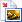
\includegraphics[width=0.6cm]{mActionExportMapServer}
 & Esporta come immagine &
 
\includegraphics[width=0.6cm]{mActionSaveAsPDF} & Esporta come PDF \\
 \hline 
\includegraphics[width=0.6cm]{mActionSaveAsSVG} & Esporta come SVG & 
\includegraphics[width=0.6cm]{mActionFilePrint}
 & Stampa \\
 \hline 
\includegraphics[width=0.6cm]{mActionZoomFullExtent} & Vista ad estensione massima & 
\includegraphics[width=0.6cm]{mActionZoomIn} & Ingrandisci \\
 \hline 
\includegraphics[width=0.6cm]{mActionZoomOut} & Rimpicciolisci &
 
\includegraphics[width=0.6cm]{mActionDraw} & Aggiorna la vista \\
 \hline 
\includegraphics[width=0.6cm]{mActionUndo} & Annulla l'ultimo cambiamento & 
\includegraphics[width=0.6cm]{mActionRedo}
 & Ripristina l'ultimo cambiamento \\
 \hline 
\includegraphics[width=0.6cm]{mActionAddMap} & Aggiungi mappa & 
\includegraphics[width=0.6cm]{mActionSaveMapAsImage}
 & Aggiungi immagine \\
  \hline 
\includegraphics[width=0.6cm]{mActionLabel} & Aggiungi etichetta & 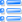
\includegraphics[width=0.6cm]{mActionAddLegend} & 
 Aggiungi nuova legenda vettoriale \\
 \hline 
\includegraphics[width=0.6cm]{mActionScaleBar} & Aggiungi nuova barra di scala
 & 
\includegraphics[width=0.6cm]{mActionAddBasicShape}
 & Aggiungi forma base \\
 \hline 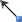
\includegraphics[width=0.6cm]{mActionAddArrow} & Aggiungi freccia
 & 
\includegraphics[width=0.6cm]{mActionOpenTable} & Aggiungi tabella attributi \\
 \hline 
\includegraphics[width=0.6cm]{mActionSelectPan} & Scegli/Sposta oggetto &
 
\includegraphics[width=0.6cm]{mActionMoveItemContent} & Sposta contenuto elemento \\
 \hline 
\includegraphics[width=0.6cm]{mActionGroupItems} & Raggruppa oggetti &
 
\includegraphics[width=0.6cm]{mActionUngroupItems} & Rimuovi raggruppamento \\
 \hline 
\includegraphics[width=0.6cm]{mActionRaiseItems} & Muovi in alto  &
 
\includegraphics[width=0.6cm]{mActionLowerItems} & Muovi in basso \\
 \hline 
\includegraphics[width=0.6cm]{mActionMoveItemsToTop} & Porta in cima &
 
\includegraphics[width=0.6cm]{mActionMoveItemsToBottom} & Sposta in fondo \\
 \hline 
\includegraphics[width=0.6cm]{mActionAlignLeft} & Allinea a sinistra &
 
\includegraphics[width=0.6cm]{mActionAlignRight} & Allinea a destra \\
 \hline 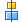
\includegraphics[width=0.6cm]{mActionAlignHCenter} & Allinea su asse verticale &
 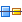
\includegraphics[width=0.6cm]{mActionAlignVCenter} & Allinea su asse orizzontale \\
 \hline 
\includegraphics[width=0.6cm]{mActionAlignTop} & Allinea in alto &
 
\includegraphics[width=0.6cm]{mActionAlignBottom} & Allinea in basso \\
\hline
\end{tabular}
\caption{Strumenti del Compositore di Stampe}\label{tab:printcomposer_tools}
\end{table}

Per accedere al compositore di stampe, cliccare sul pulsante
\toolbtntwo{mActionNewComposer}{Nuova composizione di stampa} nella barra strumenti 
o scegliere la voce di menu \mainmenuopt{File} \arrow \dropmenuopttwo{mActionNewComposer}{Nuova composizione di stampa}.

\section{Aprire un nuovo modello di stampa}\label{label_useprintcomposer} 

Prima di iniziare a lavorare con il compositore di stampe, è necessario
caricare alcuni layer raster e vettoriali nella vista mappa di QGIS e
regolarne le proprietà secondo le proprie esigenze. Una volta effettuate
tutte le impostazioni e applicata la simbologia cliccare sul pulsante
\toolbtntwo{mActionNewComposer}{Nuova composizione di stampa}.

\section{Usare il compositore di stampe}\label{label_useprintcomposer}

\begin{figure}[ht]
   \centering
   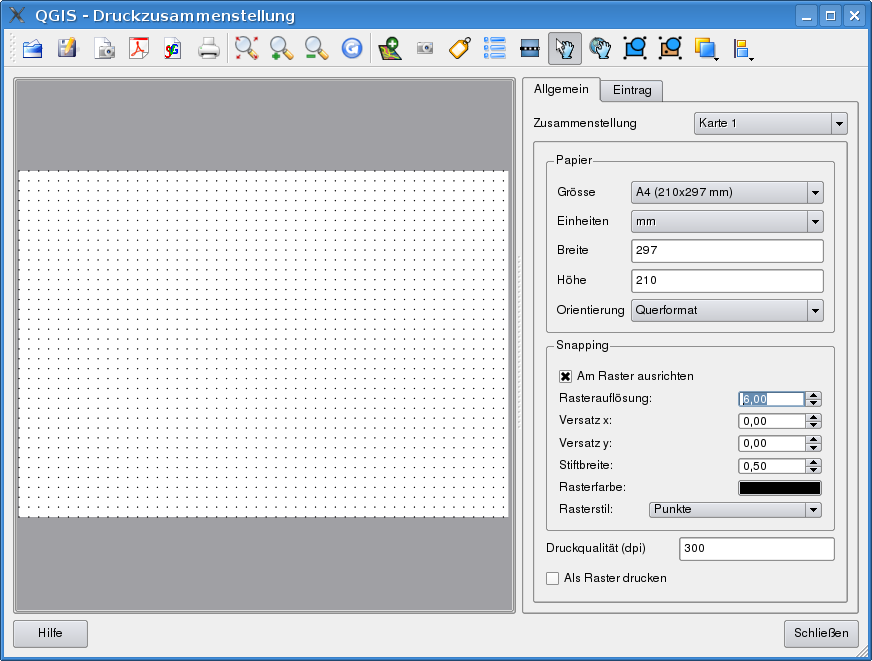
\includegraphics[clip=true, width=\textwidth]{print_composer_blank}
   \caption{Compositore di stampe \nixcaption}\label{fig:print_composer_blank}
\end{figure}

Aprendo il compositore di stampe viene visualizzato un foglio bianco al quale
aggiungere mappa, legenda, barra di scala, immagini, forme e testo. La Figura
\ref{fig:print_composer_blank} mostra la vista iniziale del compositore di
stampe prima dell'aggiunta di un qualunque elemento. 
Il compositore di stampe presenta tre schede:

\begin{itemize}[label=--]
\item La scheda \tab{Generale} consente di impostare la dimensione del
foglio, l'orientamento e la qualità di stampa del file in uscita in dpi e 
le modalità di snap. Si noti che la casella di controllo \checkbox{Snap alla griglia} 
funziona solo se si è impostata una risoluzione > 0. Inoltre, è possibile attivare 
la casella di controllo \checkbox{Stampa come raster}: tutti gli elementi saranno 
rasterizzati prima della stampa o del salvataggio come Postscript o PDF.
\item La scheda \tab{Oggetto} mostra le proprietà dell'elemento selezionato
nel layout di stampa. 
Cliccare sull'icona \toolbtntwo{mActionSelectPan}{Seleziona/Sposta oggetto} 
per selezionare un elemento (ad es. legenda, barra di scala o etichetta
testuale) nel layout. Cliccare dunque sulla scheda \tab{Oggetto} e
personalizzare le impostazioni dell'elemento selezionato.
\item La \tab{Storico comandi} mostra la storia di tutti i cambiamenti attuati nel 
layout di stampa. È possibile cancellare e ripristinare più cambiamenti con un semplice 
click del mouse.
\end{itemize}

Possono essere aggiunti diversi elementi al compositore ed è anche
possibile avere più di una mappa o legenda o barra di scala nel layout
di stampa. Ogni elemento ha le sue proprietà e, nel caso delle viste mappa, la
propria estensione. Per eliminare un elemento dal layout di stampa usare i tasti 
\keystroke{Canc} o \keystroke{backspace}.

\section{Aggiungere una mappa al layout nel compositore di stampe}

Per aggiungere una mappa, cliccare sul pulsante \toolbtntwo{mActionAddMap}{Aggiungi mappa} 
nella barra strumenti del compositore di stampe e tracciare sul layout un rettangolo in cui inserire la mappa. 
La modalità di visualizzazione della mappa può essere impostata nella scheda \tab{Oggetto}.

\begin{itemize}[label=--]
\item \selectstring{Anteprima}{Rettangolo} visualizza un rettangolo vuoto con 
la scritta \textit{"La mappa verrà stampata qui"}.
\item \selectstring{Anteprima}{Cache} disegna la mappa alla risoluzione corrente dello schermo.
 Se si ingrandisce/rimpiccolisce la finestra del compositore, la mappa non viene ridisegnata, ma 
l'immagine viene scalata.
\item \selectstring{Anteprima}{Visualizza} a differenza del metodo cache, in questo caso se si 
ridimensiona la finestra del compositore, la mappa viene ridisegnata.
\end{itemize}

\textbf{Cache} è la modalità predefinita per ogni nuovo compositore di mappe.

È possibile ridimensionare la mappa in un momento successivo cliccando sul
pulsante \toolbtntwo{mActionSelectPan}{Seleziona/Sposta oggetto}, selezionando
un elemento e trascinando una delle maniglie blu agli angoli della mappa. Una volta selezionata una mappa,
è possibile regolarne ulteriori proprietà nella scheda \tab{Oggetto}. 

Per spostare l'area visualizzata nella vista mappa,
cliccare sul pulsante \toolbtntwo{mActionMoveItemContent}{Sposta contenuto
oggetto} e spostare la vista nella cornice della vista mappa trascinando con
il tasto sinistro del mouse premuto.

È possibile \toolbtntwo{mIconLock}{bloccare/sbloccare} la posizione di un elemento 
nel layout di stampa selezionando e facendo click sullo stesso con il tasto destro del mouse, 
oppure attivando la casella di controllo \checkbox{Blocca i layer per la mappa} nella sezione 
Mappa della scheda \tab{Oggetto}.

\textbf{Nota:} QGIS \CURRENT permette di utilizzare le etichette del nuovo plugin etichette 
anche nel compositore di stampe, anche se le stesse non vengono scalate correttamente: in alcuni casi 
potrebbe essere necessario utilizzare le etichette di vecchia generazione.

\subsection{Oggetto Mappa - Mappa ed Estensione mappa}

\begin{figure}[ht]
  \centering
  \subfloat[Finestra di dialogo Mappa]{\label{subfig:map_dialog1}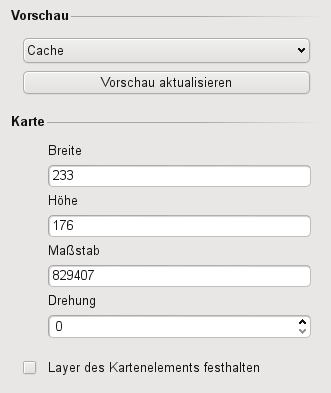
\includegraphics[clip=true, width=0.4\textwidth]{print_composer_map1}}
    \hspace{1cm}
  \subfloat[Finestra di dialogo Estensione mappa]{\label{subfig:map_dialog2}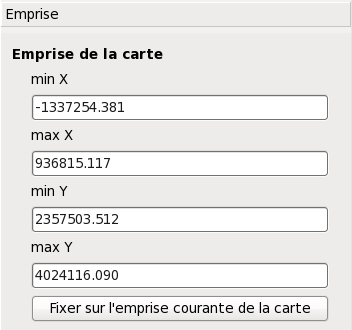
\includegraphics[clip=true, width=0.4\textwidth]{print_composer_map2}}
  \caption{Compositore di stampe - Mappa e Estensione dell'oggetto Mappa \nixcaption}\label{fig:mapdialog}
\end{figure}

\minisec{Finestra di dialogo Mappa}

La finestra di dialogo \textbf{Mappa} fornisce le seguenti funzionalità (Figura \ref{fig:mapdialog}a):

\begin{itemize}[label=--]
\item La sezione \textbf{Anteprima} permette di impostare la modalità di anteprima come descritto 
precedentemente. Cliccare su \button{Aggiorna anteprima} per salvare le modifiche.
\item La sezione \textbf{Mappa} permette di dimensionare gli elementi della mappa specificandone 
altezza e larghezza o la scala. Il campo \selectstring{Rotazione}{0} permette di ruotare il contenuto 
dell'elemento mappa in senso orario per gradi. Si noti che è possibile aggiungere un reticolato 
delle coordinate solo se il valore di rotazione è impostato a 0. Si possono, inoltre, attivare le 
caselle di controllo \checkbox{Blocca i layer per la mappa} e \checkbox{Disegna elementi sulla mappa}.
\end{itemize}

Se si apportano delle modifiche nella vista mappa di QGIS, è possibile aggiornare la vista nel 
compositore di stampe cliccando sul pulsante \button{Aggiorna anteprima}.

\minisec{Finestra di dialogo Estensione mappa}

La finestra di dialogo \textbf{Estensione mappa} fornisce le seguenti funzionalità (Figura \ref{fig:mapdialog}b):

\begin{itemize}[label=--]
\item La sezione \textbf{Estensione mappa} permette di impostare l'estensione della mappa tramite 
valori minimo/massimo in X e Y o cliccando sul pulsante \button{Imposta all'estensione della mappa}.
\end{itemize}

Se si apportano delle modifiche nella vista mappa di QGIS, è possibile aggiornare la vista nel 
compositore di stampe selezionando l'elemento mappa e cliccando sul pulsante \button{Aggiorna anteprima} 
della sezione Mappa della scheda \tab{Oggetto} (Figura~\ref{fig:mapdialog}a).

\subsection{Oggetto Mappa - Reticolato ed Opzioni generali}

\begin{figure}[ht]
\centering
   \subfloat[Finestra di dialogo Reticolato]{\label{subfig:map_dialog3}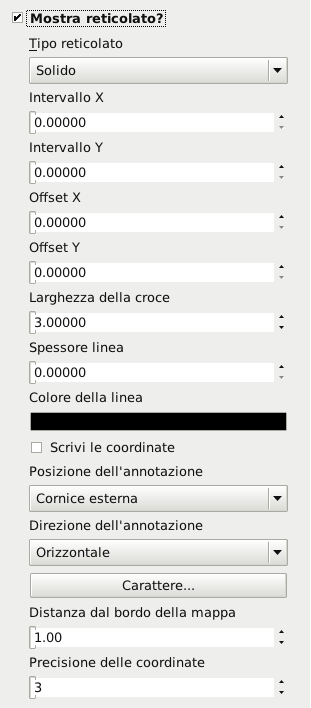
\includegraphics[clip=true, width=0.4\textwidth]{print_composer_map3}}
   \hspace{1cm}
   \subfloat[Finestra di dialogo Opzioni generali]{\label{subfig:map_dialog4}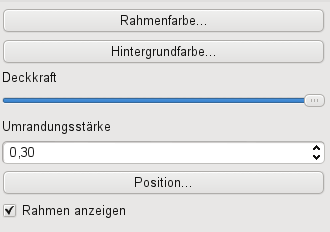
\includegraphics[clip=true, width=0.4\textwidth]{print_composer_map4}}
   \caption{Compositore di stampe - Reticolato ed Opzioni generali dell'oggetto Mappa \nixcaption}\label{fig:sec_map_dialog}
\end{figure}

\minisec{Finestra di dialogo Reticolato}

La finestra di dialogo \textbf{Reticolato} fornisce le seguenti funzionalità
(Figura \ref{fig:sec_map_dialog}a):

\begin{itemize}[label=--]
\item La casella di controllo \checkbox{Mostra reticolato} permette di sovrapporre una griglia
sull'elemento mappa, specificandone tipo (Solido o Croce), intervallo ed offset in X e Y, spessore, 
colore.
\item La casella di controllo \checkbox{Scrivi le coordinate} permette di aggiungere
le coordinate alla cornice della griglia. Le coordinate possono essere visualizzate all'interno o 
all'esterno della cornice, in verticale e/o in orizzontale; è inoltre possibile specificare il carattere,
la distanza dalla mappa e la precisione delle coordinate.
\end{itemize}

\minisec{Finestra di dialogo Opzioni generali}

Nella finestra di dialogo \textbf{Opzioni generali} (Figura \ref{fig:sec_map_dialog}b) è possibile impostare colore e spessore esterno della cornice e colore ed opacità
dello sfondo dell'elemento mappa. Il pulsante \button{Posizione e dimensione...} apre la finestra di 
dialogo \dialog{Definisci posizione oggetto} che permette di impostare la posizione dell'elemento mappa
tramite punti di riferimento o tramite coordinate.
La casella di controllo \checkbox{Mostra cornice} permette di definire se visualizzare o 
meno la cornice di un elemento.

\section{Aggiungere altri elementi al compositore di stampa} 

Oltre ad aggiungere una mappa al layout di stampa, è anche possibile
aggiungere, spostare e personalizzare legenda, barra di scala, immagini ed 
etichette.

\subsection{Oggetto etichetta - Etichetta ed Opzioni generali}

Per aggiungere un'etichetta, cliccare su \toolbtntwo{mActionLabel}{Aggiungi etichetta}, 
posizionare gli elementi con il tasto sinistro del mouse sul layout di stampa e personalizzarli 
nella scheda Etichette.

\begin{figure}[ht]
\centering
   \subfloat[Finestra di dialogo Etichetta]{\label{subfig:labeloptions1}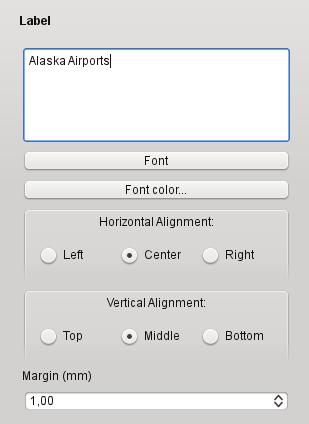
\includegraphics[clip=true, width=0.4\textwidth]{print_composer_label1}}
   \hspace{1cm}
   \subfloat[Finestra di dialogo Opzioni generali]{\label{subfig:labeloptions2}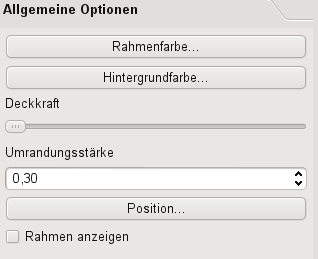
\includegraphics[clip=true, width=0.4\textwidth]{print_composer_label2}}
   \caption{Compositore di stampe - Etichetta ed Opzioni generali dell'oggetto Etichetta \nixcaption}\label{fig:label_option}
\end{figure}

\minisec{Finestra di dialogo Etichetta}

La finestra di dialogo \textbf{Etichetta} (Figura \ref{fig:label_option}a) permette di inserire un testo al layout di stampa. È possibile 
impostare allineamento, carattere, colore e margine dell'etichetta.

\minisec{Finestra di dialogo Opzioni generali}

Nella finestra di dialogo \textbf{Opzioni generali} (Figura \ref{fig:label_option}b) è possibile 
impostare colore e spessore per la cornice dell'etichetta, impostare un colore di sfondo e l'opacità. 
Il pulsante \button{Posizione e dimensione...} apre la finestra di 
dialogo \dialog{Definisci posizione oggetto} che permette di impostare la posizione dell'etichetta 
tramite punti di riferimento o tramite coordinate.
La casella di controllo \checkbox{Mostra cornice} permette di definire se visualizzare o 
meno la cornice di un elemento.

\subsection{Oggetto immagine - Opzioni immagine ed Opzioni generali}

Per aggiungere un'immagine, cliccare su \toolbtntwo{mActionSaveMapAsImage}{Aggiungi immagine},
posizionare gli elementi con il tasto sinistro del mouse sul layout di stampa e personalizzarli 
nella relativa sezione nella scheda \tab{Oggetto}.

\begin{figure}[ht]
\centering
   \subfloat[Finestra di dialogo Opzioni immagine]{\label{subfig:print_composer_image1}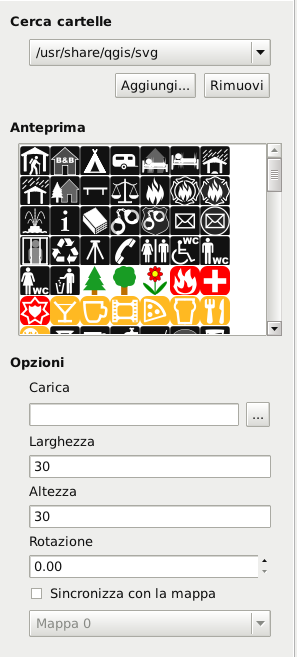
\includegraphics[clip=true, width=0.30\textwidth]{print_composer_image1}}
     \hspace{1cm}
   \subfloat[Finestra di dialogo Opzioni generali]{\label{subfig:print_composer_image2}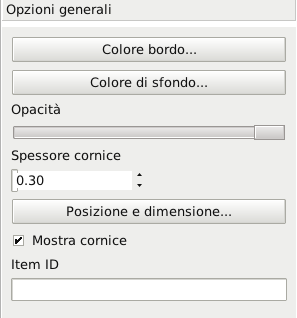
\includegraphics[clip=true, width=0.4\textwidth]{print_composer_image2}}
   \caption{Compositore di stampe - Opzioni immagine ed Opzioni generali dell'oggetto Immagine \nixcaption}\label{fig:imageoptions}
\end{figure}

\minisec{Finestra di dialogo Opzioni immagine}

La finestra di dialogo \textbf{Opzioni immagine} fornisce le seguenti funzionalità (Figura \ref{fig:imageoptions}a):

\begin{itemize}[label=--]
\item La sezione \textbf{Cerca cartelle} permettere di selezionare ed aggiungere 
alla banca dati delle immagini le cartelle contenenti immagini in formato SVG.
\item Il campo \textbf{Anteprima} mostra le immagini memorizzate nella cartella selezionata.
\item La sezione \textbf{Opzioni} permette di impostare larghezze, altezza e rotazione dell'immagine.
È possibile inserire un percorso ad un file immagine cliccando su \button{...} affianco alla casella Carica.
Attivando la casella di controllo \checkbox{Sincronizza con la mappa}, si sincronizza la rotazione 
dell'immagine con quella dell'oggetto mappa.
\end{itemize}

\minisec{Finestra di dialogo Opzioni generali}

Nella finestra di dialogo \textbf{Opzioni generali} (Figura \ref{fig:imageoptions}b) è possibile impostare colore e spessore per la cornice dell'immagine, impostare 
un colore di sfondo e l'opacità. Il pulsante \button{Posizione e dimensione...} apre la finestra di 
dialogo \dialog{Definisci posizione oggetto} che permette di impostare la posizione dell'etichetta 
tramite punti di riferimento o tramite coordinate.
La casella di controllo \checkbox{Mostra cornice} permette di definire se visualizzare o 
meno la cornice di un elemento.

\subsection{Oggetto legenda - Generale, Oggetti legenda ed Opzioni oggetto}

Per aggiungere una legenda, cliccare su \toolbtntwo{mActionAddLegend}{Aggiungi nuova legenda vettoriale},
posizionare gli elementi con il tasto sinistro del mouse sul layout di stampa e personalizzarli 
nella relativa sezione nella scheda \tab{Oggetto}.

\begin{figure}[h]
\centering
   \subfloat[Finestra di dialogo Generale]{\label{subfig:print_composer_legend1}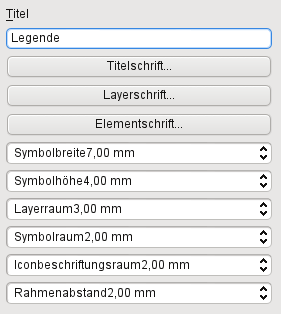
\includegraphics[clip=true, width=0.3\textwidth]{print_composer_legend1}}
   \hspace{1cm}
   \subfloat[Finestra di dialogo Oggetti legenda]{\label{subfig:print_composer_legend2}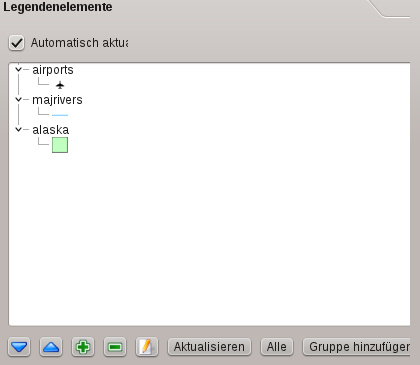
\includegraphics[clip=true, width=0.3\textwidth]{print_composer_legend2}}
   \hspace{1cm}
   \subfloat[Finestra di dialogo Opzioni oggetto]{\label{subfig:print_composer_legend3}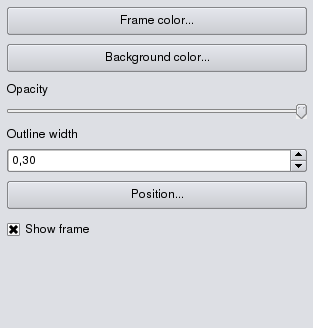
\includegraphics[clip=true, width=0.3\textwidth]{print_composer_legend3}}
   \caption{Compositore di stampe - Impostazioni dell'oggetto legenda \nixcaption}\label{fig:legendoptions}
\end{figure}

\minisec{Finestra di dialogo Generale}

La finestra di dialogo \textbf{Generale} (Figura \ref{fig:legendoptions}a) permette di inserire un titolo per la legenda ed impostare i caratteri del titolo stesso, oltre 
che dei vari elementi della legenda (layer, gruppi, etc.). È possibile cambiare dimensione ai simboli di 
legenda ed inserire layer, simboli, etichette.

\minisec{Finestra di dialogo Oggetti legenda}

La finestra di dialogo \textbf{Oggetti legenda} (Figura \ref{fig:legendoptions}b) elenca tutti gli elementi della legenda e permette di modificare (ordine e nome), 
rimuovere e ripristinare gli elementi stessi. 

Se si apportano delle modifiche alla simbologia nella vista mappa di QGIS, è possibile aggiornare 
la legenda nel compositore di stampe cliccando sul pulsante \button{Aggiorna}.
L'ordine degli elementi può essere cambiato con i pulsanti \button{Su} e \button{Giù} oppure 
trascinandoli con il mouse.

\minisec{Finestra di dialogo Opzioni oggetto}

Nella finestra di dialogo \textbf{Opzioni oggetto} (Figura \ref{fig:legendoptions}c) è possibile impostare colore e spessore per la cornice della legenda, impostare 
un colore di sfondo e l'opacità. Il pulsante \button{Posizione e dimensione...} apre la finestra di 
dialogo \dialog{Definisci posizione oggetto} che permette di impostare la posizione dell'etichetta 
tramite punti di riferimento o tramite coordinate.
La casella di controllo \checkbox{Mostra cornice} permette di definire se visualizzare o 
meno la cornice di un elemento.

\subsection{Oggetto Scala - Barra di scala ed Opzioni generali}

Per aggiungere una barra di scala, cliccare su \toolbtntwo{mActionScaleBar}{Aggiungi nuova barra di scala},
posizionare gli elementi con il tasto sinistro del mouse sul layout di stampa e personalizzarli 
nella relativa sezione nella scheda \tab{Oggetto}.

\begin{figure}[ht]
\centering
\subfloat[Finestra di dialogo Barra di scala]{\label{subfig:scalebaroptions1}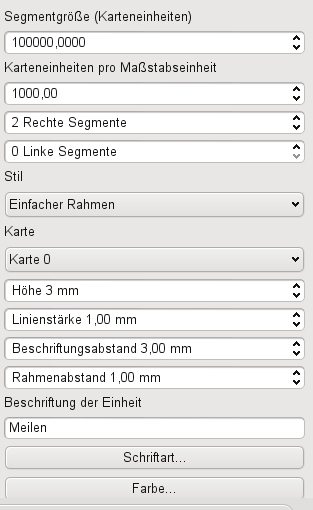
\includegraphics[clip=true, width=0.35\textwidth]{print_composer_scalebar1}}
\hspace{1cm}
\subfloat[Finestra di dialogo Opzioni generali]{\label{subfig:scalebaroptions2}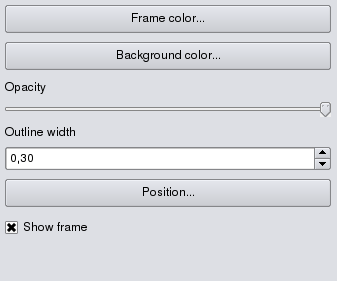
\includegraphics[clip=true, width=0.4\textwidth]{print_composer_scalebar2}}
\caption{Compositore di stampe - Impostazioni dell'oggetto Scala \nixcaption}\label{fig:scalebaroptions}
\end{figure}

\minisec{Finestra di dialogo Barra di scala} 

La finestra di dialogo \textbf{Barra di scala} fornisce le seguenti funzionalità (Figura \ref{fig:scalebaroptions}a):

\begin{itemize}[label=--]

\item Permette di impostare la dimensione del segmento della barra di scala, le unità di mappa e quanti segmenti unitari usare 
a sinistra e a destra dello 0.
\item È possibile definire lo stile della barra come riquadro singolo o doppio, con tacche verticali o numerico.
\item È possibile definire altezze, spessore linee, etichette e riquadro della barra, aggiungere etichette per l'unità di misura 
ed impostare carattere e colore.
\end{itemize}

\minisec{Finestra di dialogo Opzioni generali}

Nella finestra di dialogo \textbf{Opzioni generali} (Figura \ref{fig:scalebaroptions}b) è possibile impostare colore e spessore per la cornice della barra della scala, impostare 
un colore di sfondo e l'opacità. Il pulsante \button{Posizione e dimensione...} apre la finestra di 
dialogo \dialog{Definisci posizione oggetto} che permette di impostare la posizione dell'etichetta 
tramite punti di riferimento o tramite coordinate.
La casella di controllo \checkbox{Mostra cornice} permette di definire se visualizzare o 
meno la cornice di un elemento.

\section{Strumenti per l'esplorazione del layout di stampa}

Per l'esplorazione del layout nel compositore di stampe sono forniti quattro
strumenti:

\begin{itemize}
\item \toolbtntwo{mActionZoomFullExtent}{Vista ad estensione massima}
\item \toolbtntwo{mActionZoomOut}{Ingrandisci}
\item \toolbtntwo{mActionZoomOut}{Rimpicciolisci}
\item \toolbtntwo{mActionDraw}{Aggiorna la vista}, che serve nel caso in cui
la vista nel layout non rispecchi quanto presente nella vista mappa di QGIS. 
\end{itemize}

\section{Strumenti Annulla e Ripristina}

Durante la creazione di un layout di stampa è possibile annullare e ripristinare 
dei cambiamenti tramite gli strumenti: 

\begin{itemize}[label=--]
\item \toolbtntwo{mActionUndo}{Annulla l'ultimo cambiamento}
\item \toolbtntwo{mActionRedo}{Ripristina l'ultimo cambiamento}
\end{itemize}

oppure tramite la scheda \tab{Storico dei comandi} (Figura~\ref{fig:commandhist}).

\begin{figure}[ht]
   \centering
   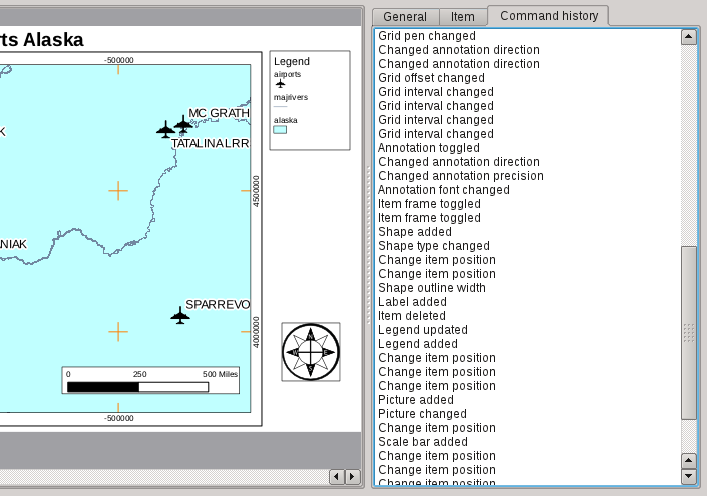
\includegraphics[clip=true, width=14cm]{command_hist}
   \caption{Storico dei comandi \nixcaption}\label
   {fig:commandhist}
\end{figure}

\section{Aggiungere forme di base e frecce}

È possibile aggiungere al layout di stampa forme geometriche (Ellisse, Rettangolo, Triangolo) e frecce.

\begin{figure}[ht]
\centering
\subfloat[Finestra di dialogo Forma]{\label{subfig:shapedialog}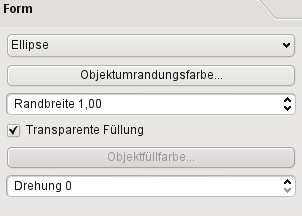
\includegraphics[clip=true, width=0.4\textwidth]{print_composer_shape}}
\hspace{1cm}
\subfloat[Finestra di dialogo Freccia]{\label{subfig:arrowdialog}\includegraphics[clip=true, width=0.4\textwidth]{print_composer_arrow}}
\caption{Compositore di stampe - Impostazioni degli oggetti Forma e Freccia \nixcaption}\label{fig:shapearrow}
\end{figure}

\begin{itemize}[label=--]
\item La finestra di dialogo \textbf{Forma} permette di tracciare un'ellisse, un rettangolo o un triangolo sul layout di stampa. 
È possibile impostare bordo, colore di riempimento e rotazione. 
\item La finestra di dialogo \textbf{Freccia} permette di tracciare una freccia sul layout di stampa.
È possibile impostare colore, bordo, spessore, indicatore.
\end{itemize}

\section{Aggiungere valori dalla tabella degli attributi}

È possibile aggiungere parti di una tabella attributi al layout di stampa.

\begin{figure}[ht]
\centering
\subfloat[Finestra di dialogo Tabella]{\label{subfig:tabledialog1}\includegraphics[clip=true, width=0.38\textwidth]{print_composer_attribute1}}
\hspace{1cm}
\subfloat[Finestra di dialogo Opzioni generali]{\label{subfig:tabledialog2}\includegraphics[clip=true, width=0.38\textwidth]{print_composer_attribute2}}
\caption{Compositore di stampe - Impostazioni dell'oggetto Tabella \nixcaption}\label{fig:attrcomp}
\end{figure}

\minisec{Finestra di dialogo Tabella}

La finestra di dialogo \textbf{Tabella} fornisce le seguenti funzionalità (Figura \ref{fig:attrcomp}a):

\begin{itemize}[label=--]
\item Permette di selezionare un layer vettoriale e le colonne della tabella degli attributi. È possibile visualizzare 
le colonne attributo in ordine crescente o decrescente. 
\item È possibile impostare il numero massimo di righe da visualizzare e scegliere se mostrare solo gli attributi 
degli elementi visibili nella mappa sul layout di stampa.
\item È, infine, possibile impostare le caratteristiche della griglia della tabella, l'intestazione ed il carattere.
\end{itemize}

\minisec{Finestra di dialogo Opzioni generali}

Nella finestra di dialogo \textbf{Opzioni generali} (Figura \ref{fig:attrcomp}b) è possibile impostare colore e spessore per la cornice della tabella, impostare 
un colore di sfondo e l'opacità. Il pulsante \button{Posizione e dimensione...} apre la finestra di 
dialogo \dialog{Definisci posizione oggetto} che permette di impostare la posizione dell'etichetta 
tramite punti di riferimento o tramite coordinate.
La casella di controllo \checkbox{Mostra cornice} permette di definire se visualizzare o 
meno la cornice di un elemento.

\section{Muovere in alto, muovere in basso ed allineare elementi}

Le funzionalità per muovere in alto o in basso gli elementi del layout di 
stampa sono nel menu \toolbtntwo{mActionRaiseItems}{Muovi gli oggetti selezionati}: 
selezionare un elemento dal layout di stampa e scegliere la funzionalità richiesta 
dal menu citato (Tabella~\ref{tab:printcomposer_tools}).

Diverse funzionalità di allineamento sono presenti nel menu 
\toolbtntwo{mActionAlignLeft}{Allinea gli oggetti selezionati} (Tabella~\ref{tab:printcomposer_tools}): selezionare alcuni elementi dal layout di 
stampa e scegliere la funzionalità richiesta dal menu citato.

\section{Creazione di file in uscita}

La Figura \ref{fig:print_composer_complete} mostra il compositore di stampe
con un layout di stampa completo di ognuno degli elementi precedentemente
descritti.

\begin{figure}[h]
   \centering
   \includegraphics[clip=true, width=\textwidth]{print_composer_complete}
   \caption{Compositore di stampe con mappa, legenda, barra della scala, coordinate e testo \nixcaption} \label{fig:print_composer_complete}
\end{figure}

Il compositore di stampe consente di creare diversi formati in uscita ed è
possibile definirne la risoluzione (qualità di stampa) e il formato pagina:

\begin{itemize}[label=--]
\item L'icona \toolbtntwo{mActionFilePrint}{Stampa} consente di stampare il
layout su una stampante collegata o su un file PDF o Postscript.
\item L'icona \toolbtntwo{mActionExportMapServer}{Esporta come immagine}
esporta il layout in diversi formati immagine come PNG, BPM, TIF, JPG, \dots
\item L'icona \toolbtntwo{mActionSaveAsPDF}{Esporta come PDF} esporta il layout in 
formato PDF.
\item L'icona \toolbtntwo{mActionSaveAsSVG}{Esporta come SVG} salva il layout
di stampa in formato SVG (Scalable Vector Graphic). \textbf{Nota:} Attualmente
il supporto SVG è ad un livello molto iniziale. Il problema non sta in QGIS,
ma nella sottostante libreria Qt. Ci si augura che questo problema venga
risolto nelle prossime versioni della libreria.
\end{itemize}

\section{Salvare e caricare un layout di stampa}

L'icona \toolbtntwo{mActionFileSaveAs}{Save come modello} consente di salvare 
lo stato della sessione del compositore di stampe come modello in un file con estensione .qpt.
L'icona \toolbtntwo{mActionFolder}{Carica dal modello} consente di caricare il modello 
salvato in un'altra sessione.

Il pulsante \toolbtntwo{mActionComposerManager}{Gestore di stampe...} nel menu \mainmenuopt{File} 
permette di aggiungere un nuovo modello di stampa e di gestire i modelli esistenti.

\begin{figure}[h]
   \centering
   \includegraphics[clip=true, width=8cm]{print_composer_manager}
   \caption{Gestore di stampe \nixcaption}
   \label{fig:print_composer_manager}
\end{figure}

\FloatBarrier
